\section{Auswertung}
\label{sec:Auswertung}

%Tabelle für den ersten Messvorgang

\begin{table}
  \centering
  \caption{Fünffache Periodendauern und Schwebungsdauer der Pendel im ersten Messvorgang}
  \label{tab:Messvorgang 1}
  \sisetup{table-format=1.2}
  \begin{tabular}{S[table-format=2.0] S S S S S S[table-format=2.2]}
      \toprule
      {Messung} & {$5T_1 \mathbin{/} \unit{\second}$} & {$5T_2 \mathbin{/} \unit{\second}$} 
      & {$5T_+ \mathbin{/} \unit{\second}$} & {$5T_- \mathbin{/} \unit{\second}$} & {$5T \mathbin{/} \unit{\second}$} & {$T_s \mathbin{/} \unit{\second}$} \\
      \midrule
       1 & 8.21 & 8.46 & 8.92 & 7.10 & 7.93 & 18.12\\  
       2 & 8.13 & 8.54 & 8.32 & 7.16 & 7.20 & 17.95\\ 
       3 & 8.30 & 8.72 & 8.26 & 7.85 & 7.94 & 18.51\\ 
       4 & 8.23 & 8.29 & 8.68 & 8.07 & 7.43 & 18.33\\ 
       5 & 8.32 & 8.66 & 8.54 & 7.60 & 8.16 & 18.36\\ 
       6 & 8.26 & 8.34 & 9.13 & 7.74 & 7.23 & 17.40\\ 
       7 & 8.25 & 8.47 & 8.04 & 7.55 & 7.71 & 18.29\\ 
       8 & 8.24 & 8.29 & 8.28 & 7.70 & 8.02 & 16.81\\ 
       9 & 8.40 & 8.62 & 8.49 & 7.83 & 7.27 & 16.99\\ 
      10 & 8.30 & 8.06 & 8.47 & 7.72 & 8.07 & 17.47\\ 
      \bottomrule
  \end{tabular}
\end{table}

Bei allen Einträgen abgesehen von der Schwebungsdauer handelt es sich um über fünf Perioden gemessene Werte, es folgt eine Tabelle mit den einfachen Periodendauern, die zwar auf drei,
aufgrund des unvermeidlichen menschlichen Fehlers bei der Messung auch auf zwei Nachkommastellen genau angegeben werden könnten. 
\newpage

\begin{table}
  \centering
  \caption{Perioden- und Schwebungsdauern der Pendel im ersten Messvorgang}
  \label{tab:Messvorgang 2}
  \sisetup{table-format=1.3}
  \begin{tabular}{S[table-format=2.0] S S S S S S[table-format=2.2]}
      \toprule
      {Messung} & {$T_1 \mathbin{/} \unit{\second}$} & {$T_2 \mathbin{/} \unit{\second}$} 
      & {$T_+ \mathbin{/} \unit{\second}$} & {$T_- \mathbin{/} \unit{\second}$} & {$T \mathbin{/} \unit{\second}$} & {$T_s \mathbin{/} \unit{\second}$} \\
      \midrule 
       1 & 1.642 & 1.692 & 1.784 & 1.420 & 1.586 & 18.12 \\  
       2 & 1.626 & 1.708 & 1.664 & 1.432 & 1.440 & 17.95 \\ 
       3 & 1.660 & 1.744 & 1.652 & 1.570 & 1.588 & 18.51 \\ 
       4 & 1.646 & 1.658 & 1.736 & 1.614 & 1.486 & 18.33 \\ 
       5 & 1.664 & 1.732 & 1.708 & 1.520 & 1.632 & 18.36 \\ 
       6 & 1.652 & 1.668 & 1.826 & 1.548 & 1.446 & 17.40 \\ 
       7 & 1.650 & 1.694 & 1.608 & 1.510 & 1.542 & 18.29 \\ 
       8 & 1.648 & 1.658 & 1.656 & 1.540 & 1.604 & 16.81 \\ 
       9 & 1.680 & 1.724 & 1.698 & 1.566 & 1.454 & 16.99 \\ 
      10 & 1.660 & 1.612 & 1.694 & 1.544 & 1.614 & 17.47 \\ 
      \bottomrule
  \end{tabular}
\end{table}

Aus diesen Messwerten lassen sich nun die einzelnen Mittelwerte und Fehler berechnen. Dabei gilt
\begin{equation}
  \bar{x}=\dfrac{1}{N}\sum_{i=1}^N x_i
\end{equation}
für den Mittelwert einer N-Messungen großen Messreihe der Größe $x$
\begin{equation}
σ=\sqrt{\dfrac{1}{N-1}\sum_{i=1}^N(x_i-\bar{x})^2}  
\end{equation}
für die Standardabweichung $σ$ und
\begin{equation}
  Δx=\dfrac{σ}{\sqrt{N}} 
\end{equation}
für die Unsicherheit $Δx$ der Messgröße $x$. \\

Für eine verknüpfte Messgröße $f(x_1,...,x_N)$ gilt die Gaußsche Fehlerfortpflanzung mit
\begin{equation}
Δf(x_1,...,x_N)=\sqrt{\sum_{i=1}^N (\frac{\partial f}{\partial x_i}Δx_i)^2}
\label{eq:gaussF}
\end{equation}


Es ergeben sich für den ersten bzw. zweiten Messvorgang:
\begin{align}
  \bar{T}_{1,1} & = x  & \bar{T}_{1,2} & = y \\
  \bar{T}_{2,1} & = x  & \bar{T}_{2,2} & = y \\ 
  \bar{T}_{+,1} & = x  & \bar{T}_{+,2} & = y \\
  \bar{T}_{-,1} & = x  & \bar{T}_{-,2} & = y \\
  \bar{T}_{,1}  & = x  & \bar{T}_{,2}  & = y \\
  \bar{T}_{S,1} & = x  & \bar{T}_{S,2} & = y 
\end{align}

Die Theoriewerte der Schwingfrequenzen sind gegeben durch

\begin{align}
  \omega   & = \frac{2π}{T}     =   \sqrt{\frac{g}{l}} \\
  \omega_+ & = \frac{2π}{T_+} =   \sqrt{\frac{g}{l}} \\
  \omega_- & = \frac{2π}{T_-} =\sqrt{\frac{g+2K}{l}} \\
  \omega_S & = \frac{2π}{T_S} =  \omega_+ -\omega_- \text{,}
\end{align}
über die Berechnung mit den Mittelwerten der Periodendauern ergeben sich die Messfrequenzen. Dabei seien die Theoriewerte durch den Index $t$
die Messfrequenzen durch den Index $m$ gekennzeichnet.

Die theoretischen Frequenzen ergeben sich zu
\begin{align}
\omega_1 & = \sqrt{\frac{g}{l_1}} = \\
\omega_2 & = \sqrt{\frac{g}{l_2}} = \\
\omega_+ & = \sqrt{\frac{g}{l}} = \\
\omega_- & = \sqrt{\frac{g+2K}{l}} = \\
\omega_S & = \omega_+ -\omega_- =
\end{align} 



\begin{figure}
  \centering
  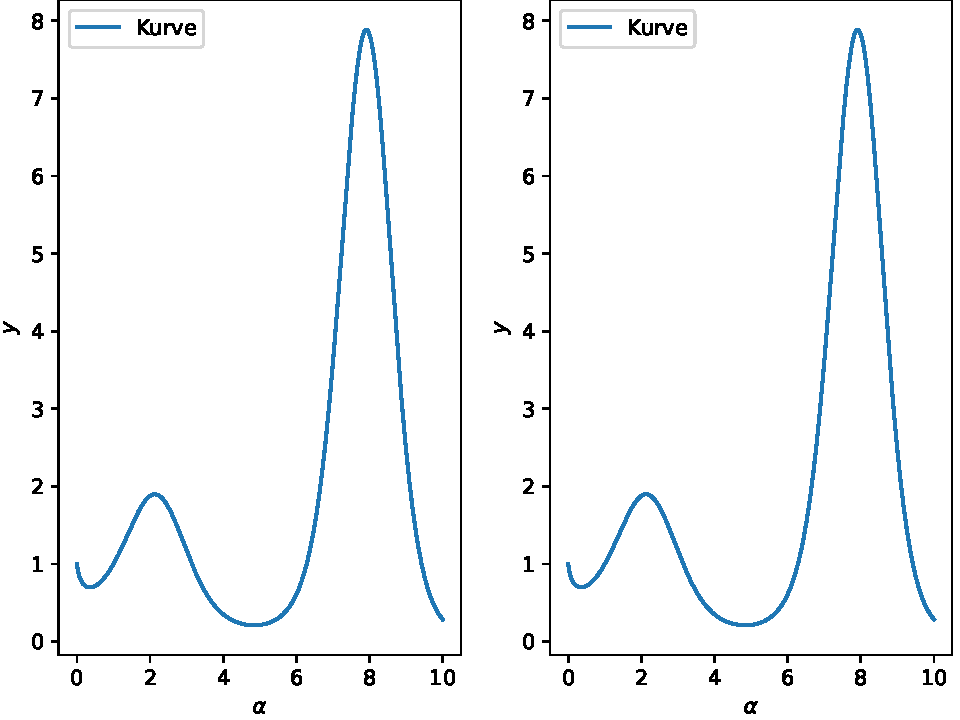
\includegraphics{plot.pdf}
  \caption{Periodendauer der beiden Pendel mit einer Pendellänge von 70 cm.}
  \label{fig:plot}
\end{figure}


%Siehe \autoref{fig:plot}! blaaaaaaaaaaaaaaaaaaaaa
